\documentclass[11pt]{article}
\usepackage[margin=1in]{geometry}
\usepackage{graphicx}
\usepackage{amsmath}
\usepackage{booktabs}

\title{A Finite Intercept Correction Calculation}
\author{Anonymous}
\date{}

\begin{document}
\maketitle

\begin{abstract}
We present a checkable worked example for learners beginning residual-based error analysis. Five synthetic observations have fixed baseline predictions \(2x\) and targets \(2x+3\). Their common residual \(3\) is removed by an intercept correction. A squared-error decomposition distinguishes minimization from exact fit, while an observation table, executable calculation, and two figures connect the arithmetic to the reuse of correction observations for evaluation.
\end{abstract}

\section{Introduction}

The instructional objective is to distinguish three ideas: selecting an empirical error minimizer, attaining zero error, and evaluating an adjustment on observations used to select it. The intended audience is learners familiar with averages and elementary algebra who are beginning to interpret prediction errors. This construction makes each distinction accessible through explicit arithmetic.

The contribution is an auditable worked example of fitting one constant with a fixed slope. Readers can trace individual observations through residual formation, correction, and evaluation, then reproduce the summary errors with the included code. The presentation connects these steps rather than treating a lower error as a self-explanatory result. The equation \(y_i=2x_i+3\) specifies the five supplied observations; it is used here within that finite construction.

\section{Related Work}

The relevant mathematical connection is between residual averaging and empirical least-squares fitting of an intercept while holding the slope at \(2\). Only one scalar changes. The comparison with absolute-error minimization below explains why the choice of objective matters, even though both objectives attain zero in this example.

The teaching sequence links observation-level arithmetic, objective functions, and evaluation dependencies. Its instructional value lies in making these connections inspectable: the table exposes every residual, the decomposition explains the correction, and the diagram shows where the targets enter both adjustment and evaluation.

\section{Method}

\subsection{Finite Setting and Residual-Mean Correction}

Table~\ref{tab:observations} contains the complete supplied observations. With fixed baseline \(\widehat y_i^{(0)}=2x_i\), define
\[
r_i=y_i-\widehat y_i^{(0)},\qquad
b=\frac{1}{5}\sum_{i=1}^{5}r_i=3,\qquad
\widehat y_i^{\,\mathrm{corr}}=2x_i+b.
\]
Every baseline residual is \(3\), so adding \(b\) reproduces each target. Figure~\ref{fig:residual_workflow} traces this deterministic calculation.

\begin{table}[htbp]
\centering
\caption{Complete supplied observations and derived residuals. The correction adds \(b=3\) to each baseline prediction.}
\label{tab:observations}
\begin{tabular}{rrrrr}
\toprule
\(x_i\) & \(y_i\) & \(2x_i\) & \(r_i\) &
\(\widehat y_i^{\,\mathrm{corr}}\) \\
\midrule
-2 & -1 & -4 & 3 & -1 \\
-1 &  1 & -2 & 3 &  1 \\
 0 &  3 &  0 & 3 &  3 \\
 1 &  5 &  2 & 3 &  5 \\
 2 &  7 &  4 & 3 &  7 \\
\bottomrule
\end{tabular}
\end{table}

\begin{figure}[htbp]
\centering
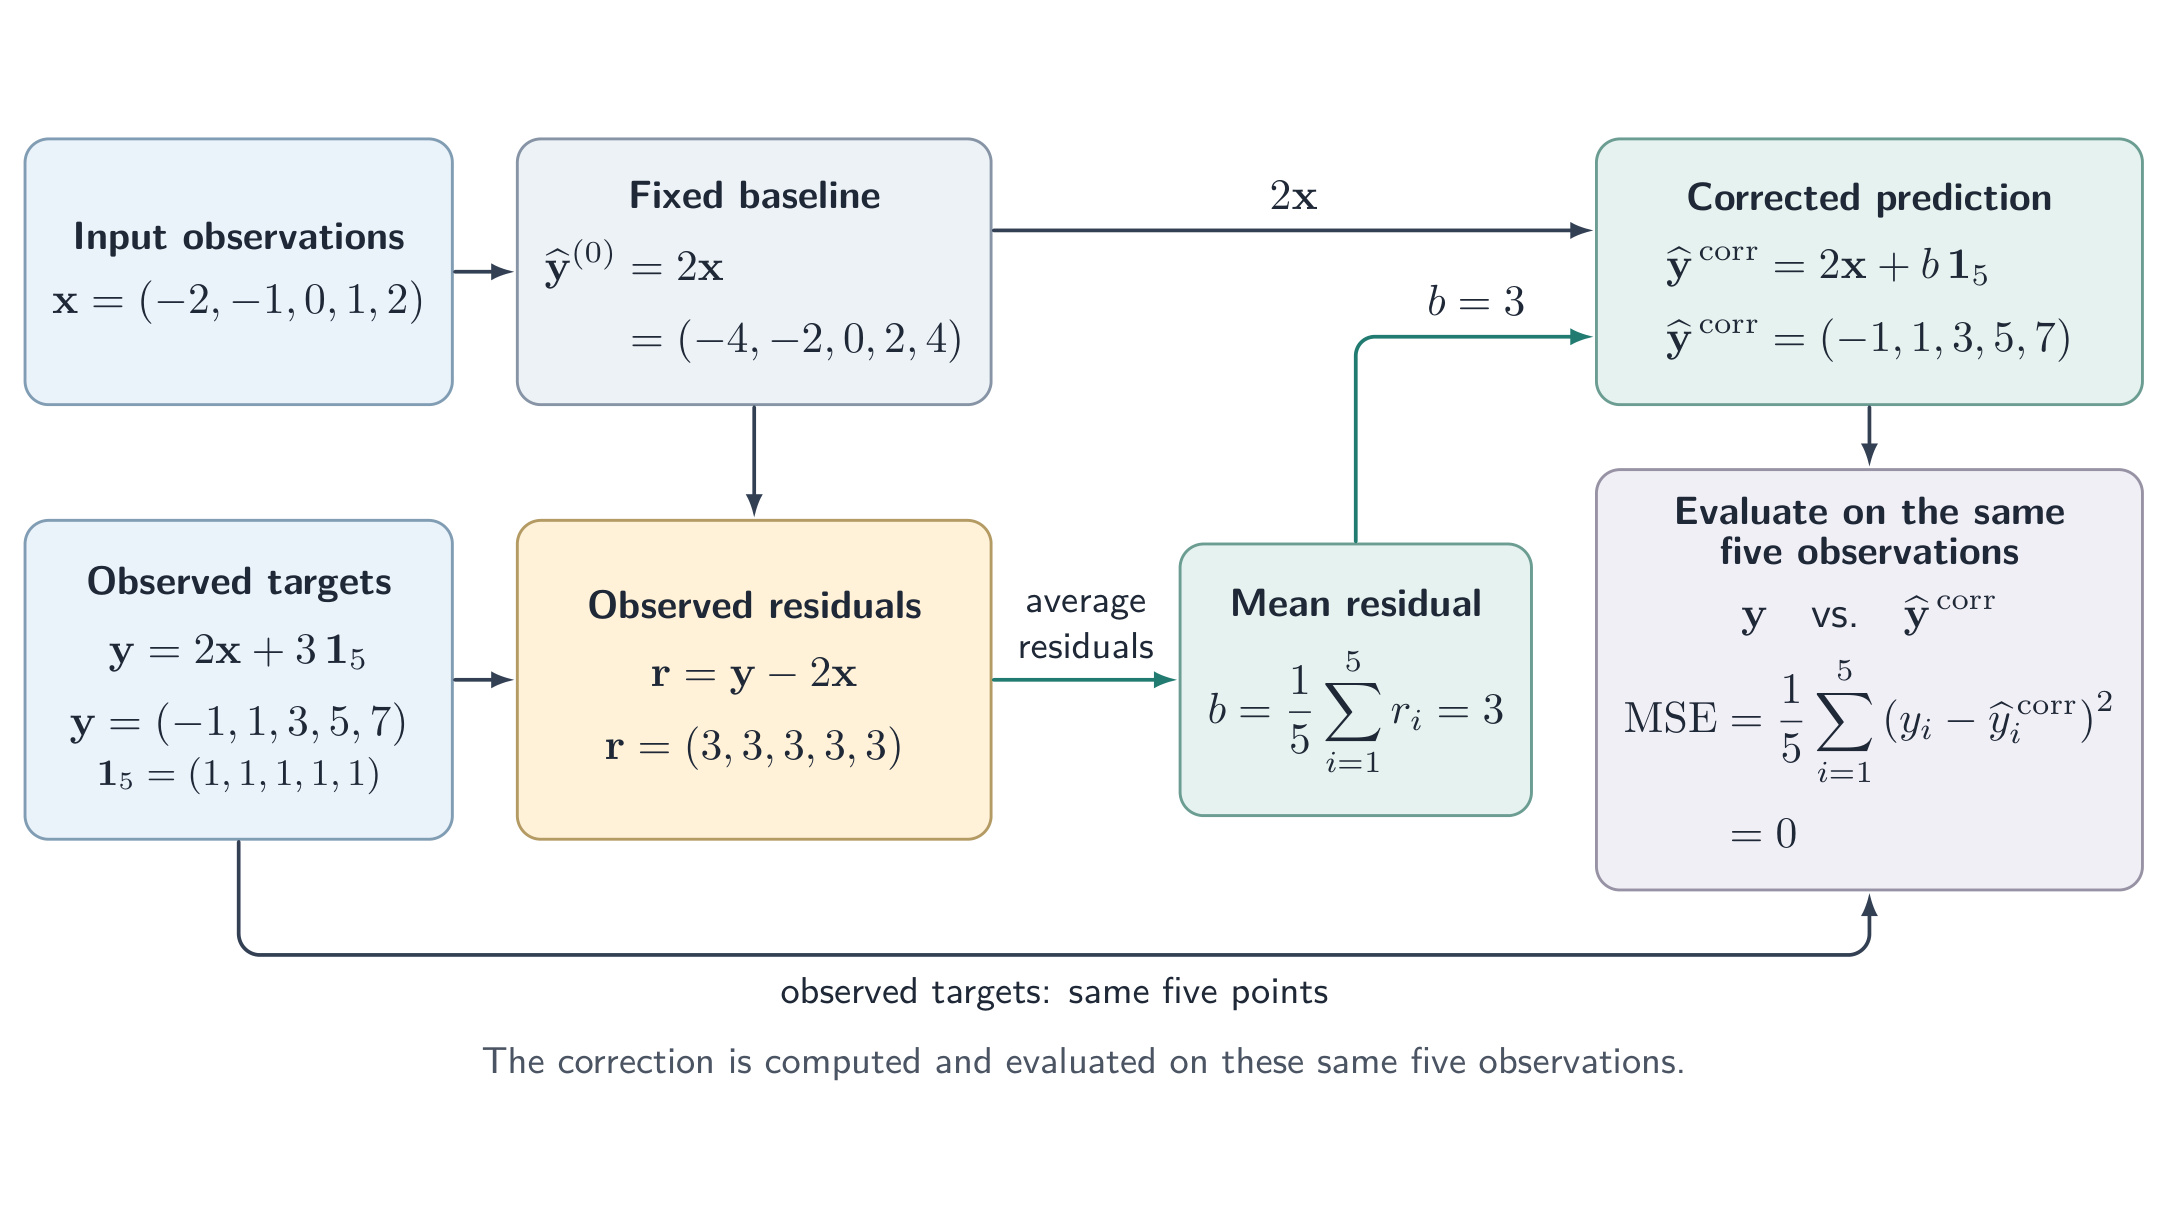
\includegraphics[width=\linewidth]{figures/fig_residual_workflow.jpg}
\caption{Dependency diagram for the supplied calculation. Identical residuals give \(b=3\); the separate path from targets to evaluation shows that the correction observations also supply the reported errors.}
\label{fig:residual_workflow}
\end{figure}

\subsection{Squared and Absolute Error}

For any finite residual vector \(r_1,\ldots,r_n\), let
\(\bar r=n^{-1}\sum_i r_i\). Expanding around its mean gives
\begin{align*}
\operatorname{MSE}(b)
&=\frac{1}{n}\sum_{i=1}^{n}(r_i-b)^2\\
&=\frac{1}{n}\sum_{i=1}^{n}(r_i-\bar r)^2
  +(b-\bar r)^2,\\
\operatorname{MSE}(0)-\operatorname{MSE}(\bar r)
&=\bar r^{\,2}.
\end{align*}
The cross term vanishes because \(\sum_i(r_i-\bar r)=0\).
Thus the mean residual minimizes empirical squared error, removing
exactly the squared mean residual from baseline MSE. The remaining
error is zero precisely when every residual equals \(\bar r\).
For nonconstant residuals, at least one positive centered squared
residual remains. These statements follow algebraically; the measured
instance here has \(n=5\).

For absolute error, order the five residuals. The sum of distances to
the smallest and largest is minimized anywhere between them; the same
holds for the second smallest and second largest. Their median lies
in both intervals and makes its own absolute residual zero. Therefore
a residual median minimizes
\(\operatorname{MAE}(b)=\frac{1}{5}\sum_i|r_i-b|\).
In the supplied calculation, mean and median both equal \(3\).

\section{Experiments}

\subsection{Calculation Setup and Reproducibility}

One deterministic base R calculation evaluates the recorded offsets
\(b=0,1.5,3\). The following executable code reproduces the correction
and error table directly from the supplied observations.

\begingroup
\small
\begin{verbatim}
x <- c(-2, -1, 0, 1, 2)
y <- c(-1, 1, 3, 5, 7)
r <- y - 2*x
b <- mean(r)
offsets <- c(0, 1.5, b)
print(data.frame(
  b = offsets,
  MAE = sapply(offsets, function(a) mean(abs(r - a))),
  MSE = sapply(offsets, function(a) mean((r - a)^2))))
\end{verbatim}
\endgroup

\subsection{Recorded Errors and Interpretation}

For these observations, the error functions simplify to
\[
\operatorname{MAE}(b)=|3-b|,
\qquad
\operatorname{MSE}(b)=(3-b)^2.
\]
Table~\ref{tab:errors} reports the recorded values. The intermediate
offset halves every residual and quarters MSE.
Figure~\ref{fig:intercept_error} displays precisely the three recorded
points.

Constant residuals explain exact fit: their centered squared residual
sum is zero. Observation reuse has a different role. The targets enter
both the choice of \(b\) and its error calculation, so these scores
describe agreement on the correction observations. The shared-target
path in Figure~\ref{fig:residual_workflow} makes this evidential context
visible without attributing the algebraic zero to reuse itself.

\begin{table}[htbp]
\centering
\caption{Recorded errors on the five correction observations.}
\label{tab:errors}
\begin{tabular}{rrr}
\toprule
Added \(b\) & Mean absolute error & Mean squared error \\
\midrule
0   & 3   & 9 \\
1.5 & 1.5 & 2.25 \\
3   & 0   & 0 \\
\bottomrule
\end{tabular}
\end{table}

\begin{figure}[htbp]
\centering
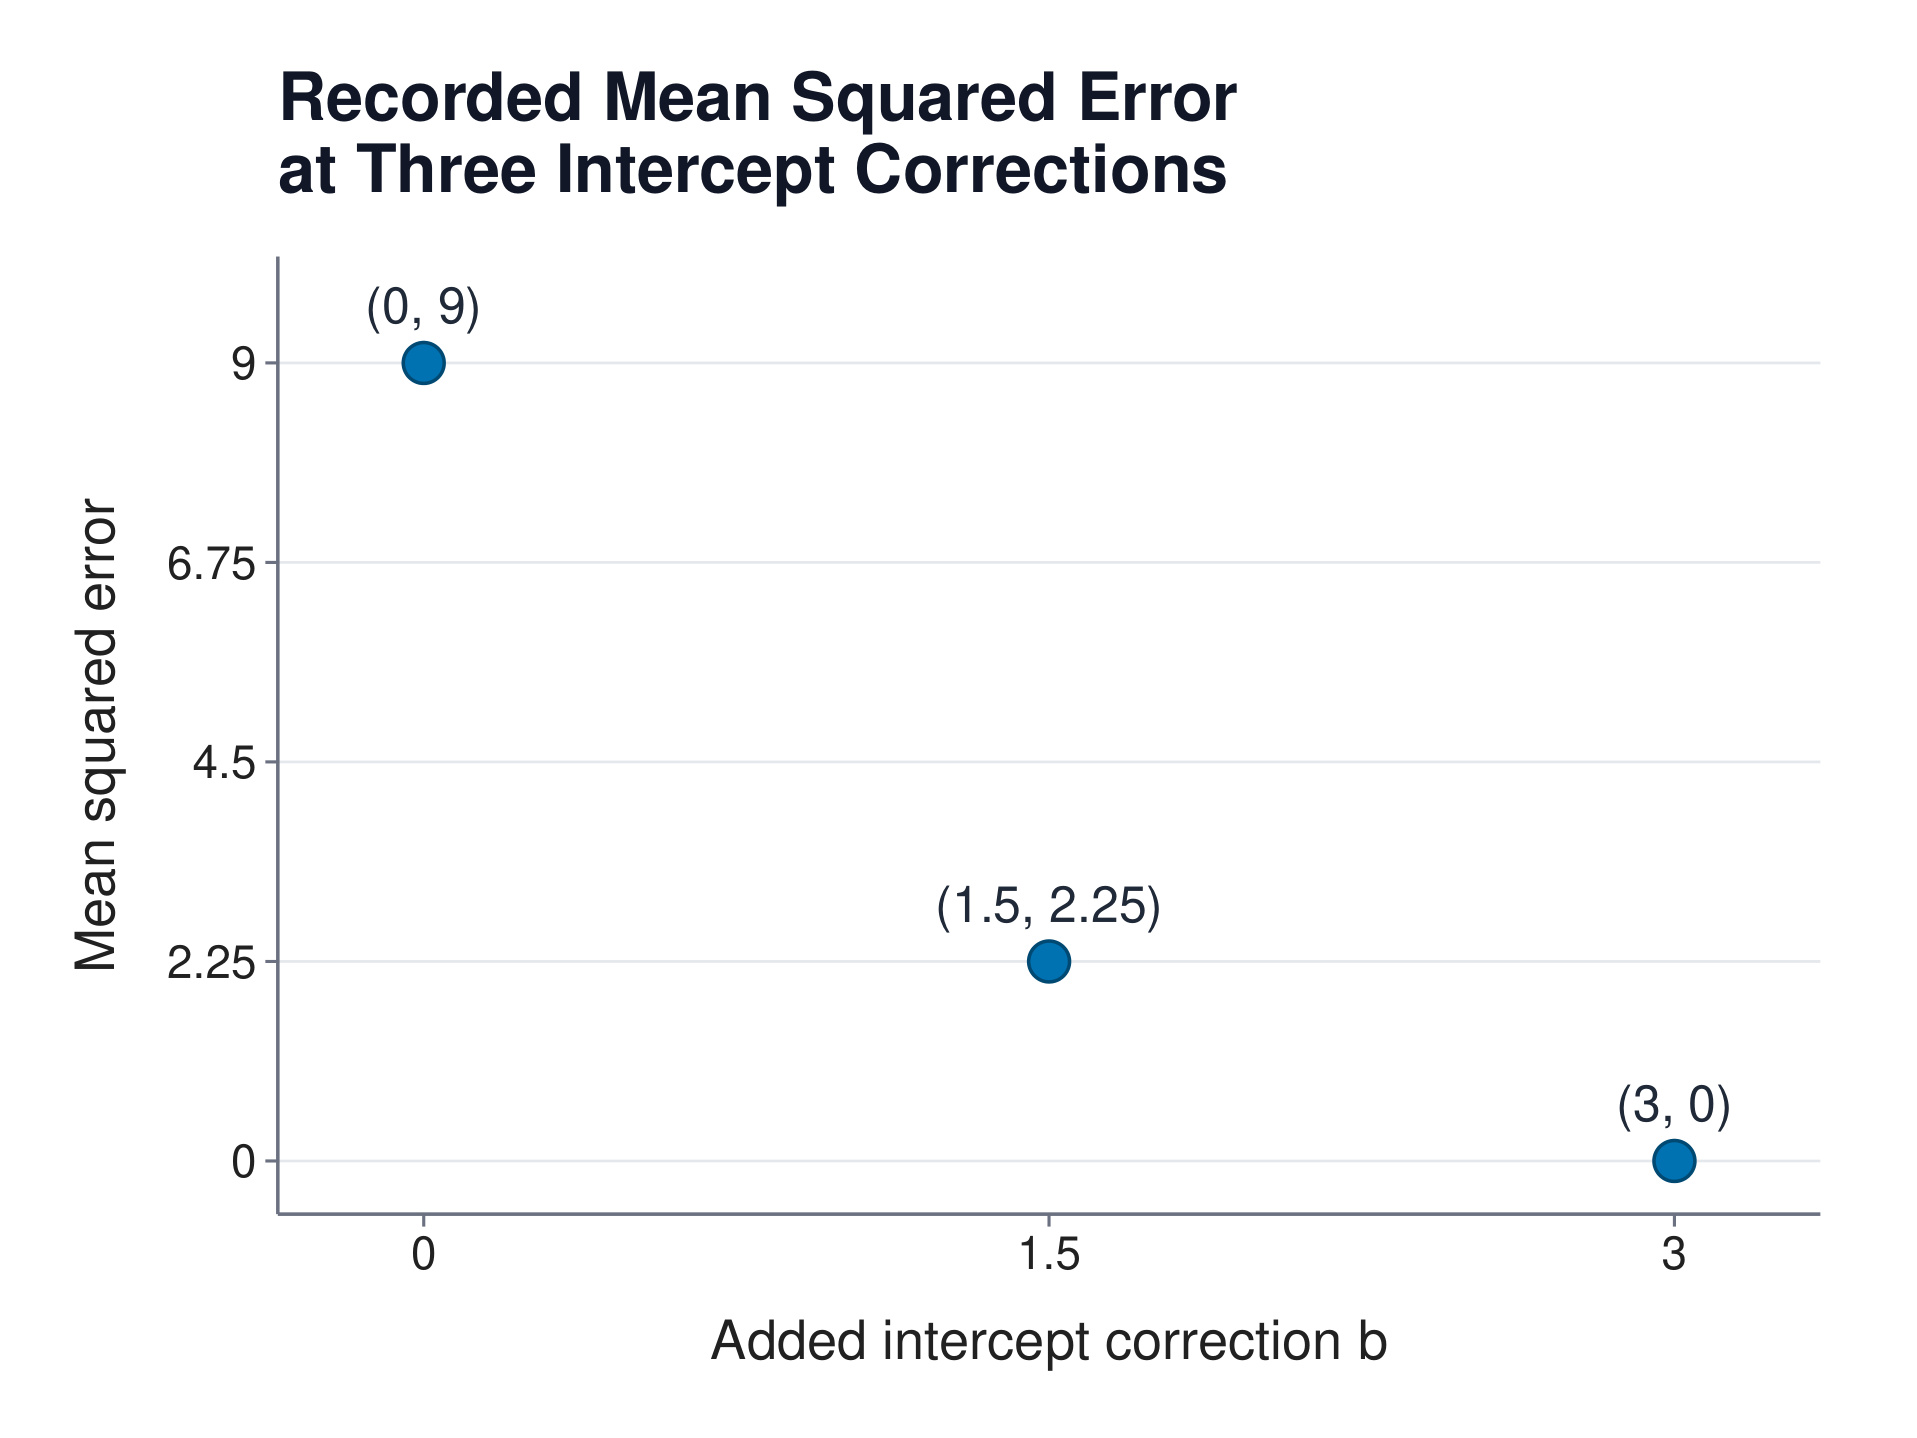
\includegraphics[width=0.78\linewidth]{figures/fig_intercept_error.jpg}
\caption{Recorded MSE at the three evaluated offsets. These points summarize the five observations in Table~\ref{tab:observations}, which also determine \(b=3\).}
\label{fig:intercept_error}
\end{figure}

\section{Conclusion}

The worked sequence connects exact arithmetic, objective-dependent
corrections, and explicit evaluation dependencies. Readers can verify
the residuals row by row and reproduce the recorded errors, while
keeping the condition for algebraic exact fit distinct from the
interpretation of scores computed on correction observations.

% PAPER_ORCHESTRA_PROVENANCE_BEGIN
\clearpage
\section*{Figure source provenance}
The files below are the exact sources that produced the embedded figure previews. Paths are relative to this manuscript's source directory. The accompanying \texttt{figure\char95{}provenance.json} records all artifact checksums.\par
\medskip\noindent\textbf{Figure~\ref{fig:intercept_error} (\texttt{fig\char95{}intercept\char95{}error.jpg}).}\par
\noindent R/ggplot2 source: \texttt{figure\char95{}code/\allowbreak{}fig\char95{}intercept\char95{}error/\allowbreak{}source.R}.\par
\noindent Source SHA256: \texttt{d2164cac\allowbreak{}bb40ae27\allowbreak{}2e285dd0\allowbreak{}123744ce\allowbreak{}d626b06c\allowbreak{}00bd67f9\allowbreak{}d17f1f86\allowbreak{}6a3da3f4}.\par
\noindent Rendering metadata: \texttt{figure\char95{}code/\allowbreak{}fig\char95{}intercept\char95{}error/\allowbreak{}render.json}.\par
\noindent Exact export wrapper: \texttt{figure\char95{}code/\allowbreak{}fig\char95{}intercept\char95{}error/\allowbreak{}worker.R}.\par
\noindent Wrapper SHA256: \texttt{6cb2b073\allowbreak{}27277f63\allowbreak{}fafbb553\allowbreak{}cd4f1f12\allowbreak{}c0f85bec\allowbreak{}37a49f3f\allowbreak{}a765da16\allowbreak{}a26b58ba}.\par
\noindent Rendering metadata: \texttt{figure\char95{}code/\allowbreak{}fig\char95{}intercept\char95{}error/\allowbreak{}sessionInfo.txt}.\par
\medskip\noindent\textbf{Figure~\ref{fig:residual_workflow} (\texttt{fig\char95{}residual\char95{}workflow.jpg}).}\par
\noindent LaTeX/TikZ source: \texttt{figure\char95{}code/\allowbreak{}fig\char95{}residual\char95{}workflow/\allowbreak{}source.tex}.\par
\noindent Source SHA256: \texttt{6f198c75\allowbreak{}4d86c280\allowbreak{}d502725d\allowbreak{}53a58390\allowbreak{}58bbbc68\allowbreak{}480fa50e\allowbreak{}e82d1dd3\allowbreak{}0cc77e65}.\par
\noindent Rendering metadata: \texttt{figure\char95{}code/\allowbreak{}fig\char95{}residual\char95{}workflow/\allowbreak{}render.json}.\par
% PAPER_ORCHESTRA_PROVENANCE_END
\end{document}